\section{Dinámicas especiales}

\subsection{Canales de Pauli}

Los canales de Pauli son canales cuánticos en los que se aplica un operador de Pauli con alguna probabilidad. El canal de Pauli de un qubit más general está definido como
\begin{gather}
    \mcP:\mcB(\hilbert_{2}) \rightarrow \mcB(\hilbert_{2})\nonumber\\
    \mcP(\Delta)=\sum_{j=0}^{3}q_{j}\pauli{j}\Delta\pauli{j}\,\text{ con }\, \sum_{j=0}^{3}q_{j}=1\rlap{.}\nonumber
\end{gather}
Reconociendo que cualquiera de los tres operadores de Pauli puede escribirse en términos de los otros dos, una manera de extender los canales de Pauli de un qubit a $n$ qubits es \cite{NPauliOperators}
\begin{gather}\label{eq:PauliChannelN}
    \mcP:\mcB(\hilbert_{2^{n}}) \rightarrow \mcB(\hilbert_{2^{n}})\nonumber\\
    \mcP(\Delta)=\sum_{\vec{j},\vec{k}}q_{\vec{j},\vec{k}}\pauli{1}^{\vec{j}}\pauli{3}^{\vec{k}}\Delta\pauli{3}^{\vec{k}}\pauli{1}^{\vec{j}}\rlap{.}
\end{gather}
donde $\pauli{j}^{\vec{k}}=\pauli{j}^{k_{1}}\otimes\pauli{j}^{k_{2}}\otimes ... \otimes \pauli{j}^{k_{n}}$ y las entradas $k_{l}$ del vector $\vec{k}$ solo pueden valer $0$ o $1$.

\subsubsection{Canales de desfasamiento}

Por canales de desfasamiento se entiende aquellos canales cuánticos cuyo efecto es amortiguar los elementos fuera de la diagonal del operador sobre el que actúan. A notar que esta definición es dependiente de la base sobre la que se está trabajando. Por ejemplo, sea $\rho\in\densityspace{2}$. Si se utiliza la base de eigenestados de $\pauli{3}$, entonces el canal
\begin{equation}
    \rho\mapsto q_{1}\rho + q_{2} \pauli{3}\rho\pauli{3}\nonumber
\end{equation}
es un canal de desfasamiento. En efecto, la acción de este canal sobre los elementos de matriz de $\rho$ es
\begin{equation}
    \begin{pmatrix}
        \rho_{0,0} & \rho_{0,1}\\
        \rho_{1,0} & \rho_{1,1}\\
    \end{pmatrix}\mapsto\begin{pmatrix}
        \rho_{0,0} & (q_{1}-q_{2})\rho_{0,1}\\
        (q_{1}-q_{2})\rho_{1,0} & \rho_{1,1}\\
    \end{pmatrix},\nonumber
\end{equation}
mientras que el canal de \textit{bit flip},
\begin{equation}
    \rho\mapsto q_{1}\rho + q_{2} \pauli{1}\rho\pauli{1},\nonumber
\end{equation}
no lo es, pues su acción sobre los elementos de matriz de $\rho$ es
\begin{equation}
    \begin{pmatrix}
        \rho_{0,0} & \rho_{0,1}\\
        \rho_{1,0} & \rho_{1,1}\\
    \end{pmatrix}\mapsto\begin{pmatrix}
        \frac{1}{2}\qty(1+(q_{1}-q_{2})(2\rho_{0,0}-1)) & \Re(\rho_{0,1})-\rmi(q_{1}-q_{2})\Im(\rho_{0,1})\\
        \Re(\rho_{1,0})+\rmi(q_{1}-q_{2})\Im(\rho_{1,0}) & \frac{1}{2}\qty(1-(q_{1}-q_{2})(1-2\rho_{1,1}))\\
    \end{pmatrix}.\nonumber
\end{equation}
Por supuesto, el canal de \textit{bit flip} es un canal de desfasamiento si se trabaja en la base de los eigenestados de $\pauli{1}$, pues en esta base, la acción del canal de \textit{bit flip} es
\begin{equation}
    \begin{pmatrix}
        \rho_{0,0} & \rho_{0,1}\\
        \rho_{1,0} & \rho_{1,1}\\
    \end{pmatrix}\mapsto\begin{pmatrix}
        \rho_{0,0} & (q_{1}-q_{2})\rho_{0,1}\\
        (q_{1}-q_{2})\rho_{1,0} & \rho_{1,1}\\
    \end{pmatrix}.\nonumber
\end{equation}
Para extender la noción de canal de desfasamiento a $n$ qubits, primero nótese que dada la base de $\hilbert_{2}$ conformada por los eigenestados de $\pauli{3}$, $\{\ket{e_{0}},\ket{e_{1}}\}$, es posible construir una base $\left\{\ket{e_{\vec{k}}}\right\}_{\vec{k}}$ de $\hilbert_{2^{n}}$ como
\begin{equation}
    \left\{\ket{e_{\vec{k}}}\right\}_{\vec{k}}=\left\{\ket{e_{\vec{k}}}\in\hilbert_{2^{n}}: \ket{e_{\vec{k}}}=\Motimes_{j=1}^{n}\ket{e_{k_{j}}},\,k_{j}\in\{0,1\}\right\} \rlap{.}\nonumber
\end{equation}
Esto es, tomando los productos tensoriales de los eigenestados de $\pauli{3}$ consigo mismos. De esta manera podemos estudiar dos canales de desfasamiento, el primero actuando en la base de productos tensoriales de eigenestados de $\pauli{3}$,
\begin{gather}
    \mcP_{\pauli{3}}:\mcB(\hilbert_{2^{n}}) \rightarrow \mcB(\hilbert_{2^{n}})\nonumber\\
    \mcP_{\pauli{3}}(\Delta)=\sum_{\vec{k}}q_{\vec{k}}\pauli{3}^{\vec{k}}\Delta\pauli{3}^{\vec{k}}\rlap{,}\nonumber
\end{gather}
que corresponde al canal de Pauli \ref{eq:PauliChannelN} cuando $\vec{j}=\vec{0}$, y el segundo definido sobre la base de productos tensoriales de eigenestados de $\pauli{1}$,
\begin{gather}
    \mcP_{\pauli{1}}:\mcB(\hilbert_{2^{n}}) \rightarrow \mcB(\hilbert_{2^{n}})\nonumber\\
    \mcP_{\pauli{1}}(\Delta)=\sum_{\vec{j}}q_{\vec{j}}\pauli{1}^{\vec{j}}\Delta\pauli{1}^{\vec{j}}\rlap{,}\nonumber
\end{gather}
que corresponde al canal de Pauli \ref{eq:PauliChannelN} cuando $\vec{k}=\vec{0}$. Es relativamente sencillo demostrar que si se escoge $q_{\vec{j}}=\frac{1-q_{\vec{0}}}{2^{n}-1}\,\forall\,\vec{j}\neq\vec{0}$, el efecto de estos canales es de reducir la amplitud de las componentes fuera de la diagonal en un factor de $(2q_{\vec{0}}-1)$. \acnote{Debe ser sencillo, el problema es que me hago bolas con los índices.} \ddnote{Ya veo lo que se necesita demostrar, hay que tener cuidado pues puede que haya $\sigma$s no triviales que conmuten con $\sigma_1 \otimes \sigma_1 \otimes \dots$, o aclarame, solo hay productos de $\sigma_1$ e identidades?}

Consideremos entonces en canal de desfasamiento de dos qubits en cualquiera de las dos direcciones discutidas y con probabilidades como mencionadas anteriormente. Sea $\rho_{\ef}$ un estado efectivo en $\densityspace{2}$ correspondiente a un sistema $\varrho \in \densityspace{2^{n}}$, y sea $\varrho_{\max}\in\densityspace{2^{n}}$ el estado de máxima entropía compatible con el estado efectivo. Si se propaga al estado de máxima entropía por medio de este canal y luego se pasa el resultado por la aplicación de grano grueso, el resultado es una dinámica efectiva
\begin{equation}
  \Gamma_{t}(\rho_{\ef})=\mcC\qty[\sum_{\vec{j}}q_{\vec{j}}\,\pauli{3}^{\vec{j}}\varrho_{\max}\pauli{3}^{\vec{j}}]=\mcC\qty[\sum_{\vec{j}}q_{\vec{j}}\,\qty(\Motimes_{k=1}^{n} \pauli{3}^{j_{k}}\rho_{k}\pauli{3}^{j_{k}})]\nonumber.\nonumber
\end{equation}
Para resolver el lado derecho de la ecuación, nótese que existen $2^{n}$ posibles vectores $\vec{j}$, y dentro de estos, $2^{n-1}$ tienen un $0$ o un $1$ en la $\nu$-ésima posición. Esto significa que hay $\frac{2^{n-1}}{n}$ ceros y $\frac{2^{n-1}}{n}$ unos en cada posible entrada de todos los $\vec{j}$. Entonces podemos usar el hecho de que tanto los operadores $\pauli{3}^{\vec{j}}$ como el estado de máxima entropía son factorizables, así como que la aplicación de grano es lineal para sumar sobre dichos ceros y unos:
\begin{align}
    \mcC\qty[\sum_{\vec{j}}q_{\vec{j}}\,\qty(\Motimes_{k=1}^{n} \pauli{3}^{j_{k}}\rho_{k}\pauli{3}^{j_{k}})]=&\sum_{\vec{j}}q_{\vec{j}}\sum_{k=1}^{n}p_{k}\pauli{3}^{j_{k}}\rho_{k}\pauli{3}^{j_{k}}\nonumber\\
    =&\sum_{\{j_{k}:j_{k}=0\}}q_{j_{k}}\sum_{k=1}^{n}p_{k}\pauli{3}^{j_{k}}\rho_{k}\pauli{3}^{j_{k}}+\sum_{\{j_{k}:j_{k}=1\}}q_{j_{k}}\sum_{k=1}^{n}p_{k}\pauli{3}^{j_{k}}\rho_{k}\pauli{3}^{j_{k}}\nonumber\\
    =&q_{\vec{0}}\qty(\sum_{k=1}^{n}p_{k}\rho_{k})+\frac{1-q_{\vec{0}}}{2^{n}-1}(2^{n-1}-1)\qty(\sum_{k=1}^{n}p_{k}\rho_{k})+\frac{1-q_{\vec{0}}}{2^{n}-1}2^{n-1}\qty(\sum_{k=1}^{n}\pauli{3}p_{k}\rho_{k}\pauli{3}).\nonumber
\end{align}
Con lo que la dinámica efectiva es
\begin{equation}
    \Gamma_{t}(\rho_{\ef})=\qty(q_{\vec{0}}+\frac{2^{n-1}-1}{2^{n}-1}(1-q_{\vec{0}}))\rho_{\ef}+\qty(\frac{2^{n-1}}{2^{n}-1}(1-q_{\vec{0}}))\pauli{3}\rho_{\ef}\pauli{3}.\nonumber
\end{equation}
Nótese que la dinámica efectiva es lineal, y que únicamente depende de del número de partículas en el sistema microscópico. Aún más, este es un canal de desfasamiento de un qubit en dirección de $\pauli{3}$. Este resultado es análogo para el canal $P_{\pauli{1}}$. Para recuperar un canal de desfasamiento total (en el que todos los elementos fuera de la diagonal se hacen cero) basta con elegir $q_{\vec{j}}=\frac{1}{2^{n}}\,\forall\,\vec{j}$. En dicho caso la dinámica efectiva se reduce a
\begin{equation}\label{eq:EffectiveDephasing}
    \Gamma_{t}(\rho_{\ef})=\frac{1}{2}(\rho_{\ef}+\pauli{3}\rho_{\ef}\pauli{3}).
\end{equation}
Esto es, el desfasamiento total en $n$ partículas se traduce como un desfasamiento total en una partícula.


\subsubsection{Canal de despolarización}

El canal de despolarización es el canal cuántico que contrae de manera uniforme a todos los estados hacia el estado máximamente mezclado. Al canal de despolarización se le define como
\begin{gather}\label{eq:DepolarizingChannelN}
    \mcD_{q}:\mcB(\hilbert_{2^{n}}) \rightarrow \mcB(\hilbert_{2^{n}})\nonumber\\
    \mcD_{q}(\Delta)=q\Delta+(1-q)\Id_{2^{n}}\Tr(\Delta)\rlap{.}
\end{gather}
Ahora, nótese que el canal de despolarización total puede verse como una concatenación de dos canales de desfasamiento total, uno en dirección $\pauli{1}$ y luego otro en dirección $\pauli{3}$ (el orden es irrelevante). Para ver esto, es particularmente útil escribir a la matriz de densidad $\varrho\in\densityspace{2^{n}}$ en términos de las componentes de su vector de Bloch,
\begin{equation}
    \varrho=\frac{1}{2^{n}}\sum_{\vec{j},\vec{k}}\gamma_{\vec{j},\vec{k}}\pauli{1}^{\vec{j}}\pauli{3}^{\vec{k}},\nonumber
\end{equation}
y notar que el efecto de dichos canales se puede ver como
\begin{align}
    \mcP_{\pauli{1}}(\varrho)=\frac{1}{2^{n}}\sum_{\vec{j},\vec{k}}\delta_{\vec{k},\vec{0}}\gamma_{\vec{j},\vec{k}}\pauli{1}^{\vec{j}}\pauli{3}^{\vec{k}}  & & \text{y} & & \mcP_{\pauli{3}}(\varrho)=\frac{1}{2^{n}}\sum_{\vec{j},\vec{k}}\delta_{\vec{j},\vec{0}}\gamma_{\vec{j},\vec{k}}\pauli{1}^{\vec{j}}\pauli{3}^{\vec{k}} \nonumber
\end{align}
de tal forma que su composición es
\begin{align}
    \qty(\mcP_{\pauli{1}}\circ \mcP_{\pauli{3}})(\varrho)&=\frac{1}{2^{n}}\sum_{\vec{j},\vec{k}}\delta_{\vec{j},\vec{0}}\delta_{\vec{k},\vec{0}}\gamma_{\vec{j},\vec{k}}\pauli{1}^{\vec{j}}\pauli{3}^{\vec{k}}\nonumber\\
    &=\frac{1}{2^{n}}\gamma_{\vec{0},\vec{0}}\Id_{2^{n}}.\nonumber
\end{align}
Que es precisamente el efecto del canal de despolarización total. Ahora, sea $\rho_{\ef}$ un estado efectivo en $\densityspace{2}$ correspondiente a un sistema $\varrho \in \densityspace{2^{n}}$, y sea $\varrho_{\max}\in\densityspace{2^{n}}$ el estado de máxima entropía compatible con el estado efectivo. Es inmediato ver que la dinámica efectiva correspondiente a un canal de despolarización total es otro canal de despolarización total, i.e.
\begin{equation}
    \Gamma_{t}(\rho_{\ef})=\frac{1}{2}\Id_{2}.
\end{equation}
Ahora, sabiendo que
\begin{equation}
    \qty(\mcP_{\pauli{1}}\circ \mcP_{\pauli{3}})(\varrho)=\frac{1}{2^{2n}}\sum_{\vec{j},\vec{k}}\pauli{1}^{\vec{j}}\pauli{3}^{\vec{k}}\varrho\pauli{3}^{\vec{k}}\pauli{1}^{\vec{j}}=\frac{1}{2^{n}}\Id_{2^{n}}\nonumber
\end{equation}
la ecuación \ref{eq:DepolarizingChannelN} puede reescribirse como
\begin{equation}
    \mcD_{q}(\varrho)=\frac{q(2^{2n}-1)+1}{2^{2n}}\varrho+\frac{(1-q)}{2^{2n}}\sum_{\vec{j}\land\vec{k}\neq\vec{0}}\pauli{1}^{\vec{j}}\pauli{3}^{\vec{k}}\varrho\pauli{3}^{\vec{k}}\pauli{1}^{\vec{j}}\nonumber
\end{equation}
Donde es explícitamente claro que el canal de despolarización es un canal de Pauli. La dinámica efectiva que corresponde al canal de despolarización no completo es simplemente
\begin{equation}\label{eq:EffectiveDepolarizing}
    \Gamma_{t}(\rho_{\ef})=q\rho_{\ef}+(1-q)\Id_{2}.
\end{equation}
Esto es, la dinámica efectiva correspondiente a un canal de despolarización siempre es un canal de despolarización. Nótese que este resultado es muy similar al obtenido para una evolución unitaria subyacente generada por un Hamiltoniano de la forma $\mcH=H\otimes\Id+\Id\otimes H$. En dicho caso, la dinámica efectiva era, justamente, la unitaria generada por el Hamiltoniano $H$, esto como consecuencia de la simetría de la evolución: la misma para cada partícula, sin interacción. Este caso es el mismo, el canal de despolarización actúa de la misma forma sobre cada partícula, y es completamente isotrópico dentro del subespacio de cada partícula.

\subsection{Canal de estabilización}

El canal de amortiguamiento de amplitud funciona como un modelo simple de emisión espontánea. En efecto, un átomo de dos niveles acoplado a un campo electromagnético experimenta emisión espontánea, y puede demostrarse que este proceso corresponde a un canal de amortiguamiento de amplitud si se traza al campo y se considera que la frecuencia del campo es igual a la frecuencia de resonancia de transiciones entre los niveles del átomo \cite{Fox}. El canal de amortiguamiento de amplitud tiene el efecto de enviar todos los estados al estado base. Aquí estudiaremos un canal más sencillo, que envía todos los estados a un estado puro dado $\ket{\psi}$ de forma exponencial en el tiempo, como si el átomo de dos niveles tendiera a estabilizarse en dicho estado.

Considérese entonces que un sistema de $n$ partículas evoluciona siguiendo el canal cuántico
\begin{gather}
    \mcE_{\psi,t}:\mcB(\hilbert_{2^{n}}) \rightarrow \mcB(\hilbert_{2^{n}})\nonumber\\
    \mcE_{\psi,t}(\Delta)=e^{-t\mu}\varrho+(1-e^{-t \mu})\dyad{\psi}\Tr(\Delta)\rlap{.}\nonumber
\end{gather}
donde $\dyad{\psi}\in \densityspace{2^{n}}$. Es importante señalar que si se escoge $n=1$ y $\ket{\psi}=\ket{0}$ no se recupera el canal de amortiguamiento de amplitud, pues el canal de amortiguamiento de amplitud tiene el siguiente efecto sobre la matriz de densidad
\begin{equation}
    \begin{pmatrix}
        \rho_{0,0} & \rho_{0,1} \\
        \rho_{1,0} & \rho_{1,1}
    \end{pmatrix}\mapsto\begin{pmatrix}
        (1-\gamma)\rho_{0,0}+\gamma & \sqrt{1-\gamma}\rho_{0,1} \\
        \sqrt{1-\gamma}\rho_{1,0} & (1-\gamma)\rho_{1,1}
    \end{pmatrix},\nonumber
\end{equation}
donde $\gamma$ puede verse como la probabilidad de emisión de un fotón, mientras que el canal $\mcE_{\ket{0},t}$ tiene el efecto
\begin{equation}
    \begin{pmatrix}
        \rho_{0,0} & \rho_{0,1} \\
        \rho_{1,0} & \rho_{1,1}
    \end{pmatrix}\mapsto\begin{pmatrix}
        (1-\gamma)\rho_{0,0}+\gamma & (1-\gamma)\rho_{0,1} \\
        (1-\gamma)\rho_{1,0} & (1-\gamma)\rho_{1,1}
    \end{pmatrix}.\nonumber
\end{equation}
donde se ha hecho $e^{\mu t}=\gamma$. Es claro que el canal de amortiguamiento y el canal de estabilización tienen efectos diferentes en las fases del estado. Aún más, mientras que la extensión del canal de estabilización a $n$ partículas es directa, la generalización del canal de amortiguamiento de amplitud es no trivial, ya que no hay una forma única de conectar los amortiguamientos entre los niveles energéticos.

Ahora, sea $\rho_{\ef}$ un estado efectivo en $\densityspace{2}$ y $\varrho_{\max}$ el estado de máxima entropía en $\densityspace{2^{n}}$ compatible con este. Aplicando el modelo de grano grueso al estado de máxima entropía propagado por el canal de estabilización se obtiene que
\begin{equation}\label{eq:EffectiveStabilizing}
    \Gamma_{t}(\rho_{\ef})=e^{-t\mu}\rho(0)+(1-e^{-t \mu})\mcC(\dyad{\psi}).\nonumber
\end{equation}
Obsérvese que la dinámica efectiva es un canal cuántico, pero no necesariamente un canal de estabilización, pues el estado al que tiende el sistema efectivo, $\mcC(\dyad{\psi})$ no tiene por qué ser un estado puro. En realidad, en el caso en que $\ket{\psi}$ es un estado máximamente entrelazado, $\mcC(\dyad{\psi})$ es el estado máximamente mezclado, de tal manera que la dinámica efectiva es un canal de despolarización.

\subsection{Cadena de espines de Heisenberg}

\ddnote{Ok, a esta no le he puesto atención, como me dijiste}

El modelo $XZY_{s}$ unodimensional de Heisenberg consiste en una cadena de $n$ partículas de espín $s$ en la que se consideran interacciones de espín entre primeros vecinos. Se ha demostrado que la cadena de Heisenberg describe el comportamiento de algunos metales y cristales \cite{HeisenbergModel}. El hamiltoniano del modelo de Heisenberg en el caso de espín $\frac{1}{2}$ es
\begin{equation}
    \mcH=\sum_{k=1}^{n}\qty(J_{1}\pauli{1,k}\pauli{1,k+1}+J_{2}\pauli{2,k}\pauli{2,k+1}+J_{3}\pauli{3,k}\pauli{3,k+1})-g\sum_{k=1}^{n}\pauli{2,k},
\end{equation}
donde $J_{k}$ son las constantes de acoplamiento, $\pauli{j,k}$ es el operador de Pauli $j$ que actúa sobre la $k$-ésima partícula, y $g$ es la constante del campo transversal. Existen diferentes simplificaciones que pueden hacerse del modelo de Heisenberg. La primera es el caso $J_{1}=J_{2}=J_{3}$, llamado modelo $XXX_{\frac{1}{2}}$. La segunda es considerar que las interacciones entre las partículas se da únicamente en la dirección de $\pauli{3}$, que corresponde al modelo unidimensional de Ising. Además, en ambos casos es posible hacer nulo el campo transversal, i.e. $g=0$

\subsubsection{Modelo de Ising}

Como primer ejemplo, considérese el modelo de Ising sin campo transversal (i.e. $g=0$). En este caso, el hamiltoniano se reduce a
\begin{equation}
    \mcH=\omega\sum_{k=1}^{n-1}\pauli{3,k}\pauli{3,k+1}.\nonumber
\end{equation}
si la cadena es abierta (ver figura \ref{fig:IsingChainOpen}). Para que la cadena sea cerrada (ver figura \ref{fig:IsingChainClosed}) basta con añadir el término de interacción entre la primera y la $n$-ésima partícula,
\begin{equation}
    \mcH=\omega\qty(\pauli{3,1}\pauli{3,n}+\sum_{k=1}^{n-1}\pauli{3,k}\pauli{3,k+1}).\nonumber
\end{equation}
\begin{figure}[ht!]
    \centering
    \begin{subfigure}{0.5\textwidth}
      \centering
      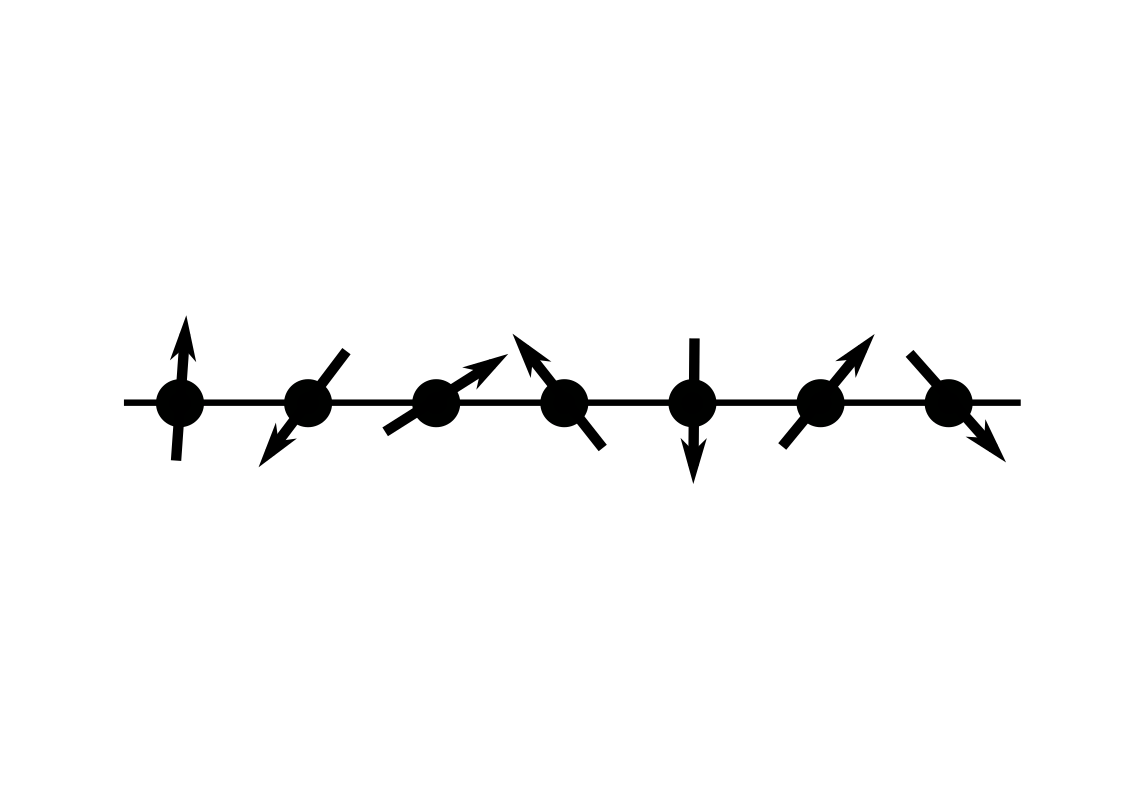
\includegraphics[width=0.7\linewidth]{chapter3/figures_special/OpenIsing.png}
      \caption{Cadena de Ising abierta. \label{fig:IsingChainOpen}}
    \end{subfigure}%
    \begin{subfigure}{0.5\textwidth}
      \centering
      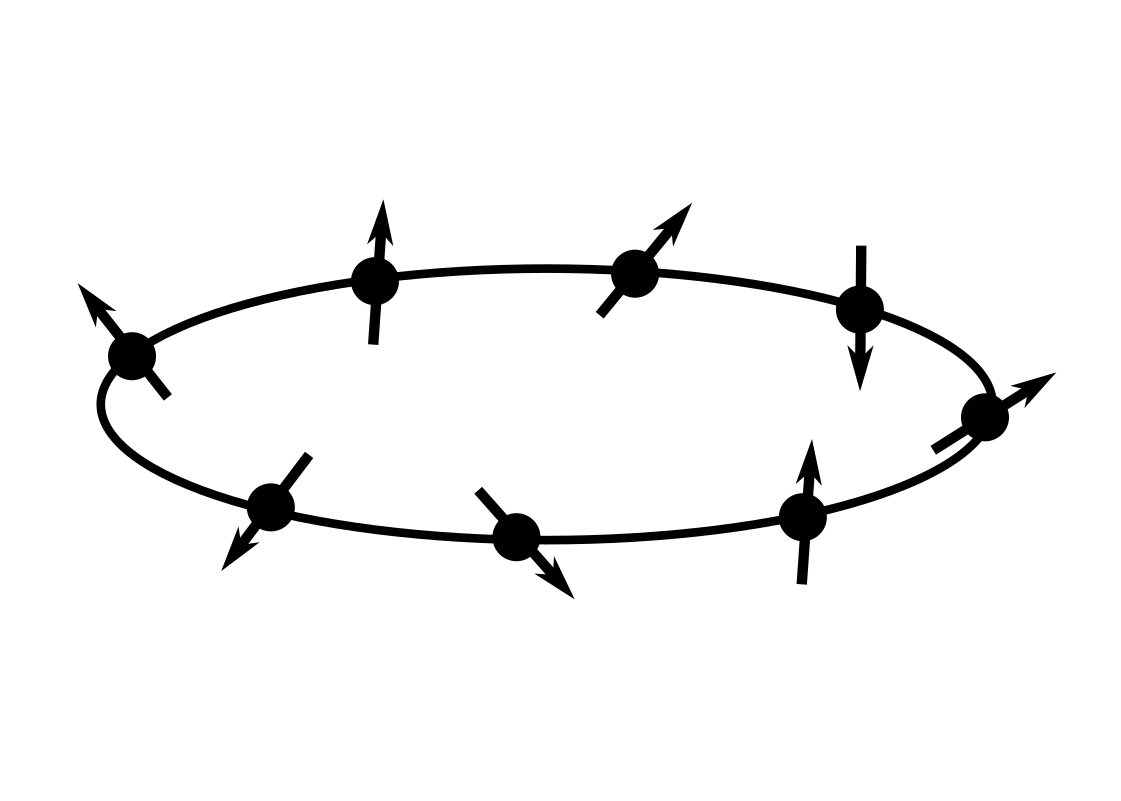
\includegraphics[width=0.7\linewidth]{chapter3/figures_special/ClosedIsing.png}
      \caption{Cadena de Ising cerrada. \label{fig:IsingChainClosed}}
    \end{subfigure}
    \caption{Diagrama de la cadena de Ising. \label{fig:IsingChainOpenAndClosed}}
    
\end{figure}
Sea entonces $\rho_{\ef}\in\densityspace{2}$ un estado efectivo correspondiente a un sistema de $n=2$ partículas, y $\varrho_{\max}$ el estado microscópico compatible con $\rho_{\ef}$ que maximiza la entropía. El hamiltoniano del sistema microscópico es, explícitamente,
\begin{equation}
    \mcH=\omega\qty(\pauli{3}\otimes\pauli{3}),\nonumber
\end{equation}
de tal forma que dicho sistema evoluciona de acuerdo al operador unitario
\begin{equation}
    \mcU_{t}=\Id \cos(\omega t)+ \rmi \pauli{3}\otimes\pauli{3} \sin(\omega t).\nonumber
\end{equation}
Si se propaga al estado de máxima entropía con dicho operador y se le pasa por la aplicación de grano grueso, la dinámica efectiva es
\begin{align}
    \Gamma_{t}(\rho_{\ef})=&\rho_{\ef} \cos^{2}(\omega)+\pauli{3} \rho_{\ef} \pauli{3} \sin^{2}(\omega t)\nonumber\\
    & + \rmi \sin(\omega t)\cos(\omega t)\qty(p_{1}\expval{\pauli{3}}_{2}[\pauli{3},\rho_{1}]+p_{2}\expval{\pauli{3}}_{1}[\pauli{3},\rho_{2}]).\nonumber
\end{align}
Dentro de la expresión de la dinámica efectiva reconocemos dos términos. El primero es un canal de desfasamiento sobre el estado efectivo, mientras que el segundo depende tanto de los parámetros de la aplicación de grano grueso, $p_{1}$ y $p_{2}$, como de valores esperados con respecto a los operadores de densidad reducidos del estado de máxima entropía. En efecto, el caso límite $p_{1}=1$ ve la dinámica efectiva reducida a un canal de desfasamiento en el tiempo,
\begin{equation}\label{eq:EffectiveIsing2}
    \Gamma_{t}(\rho_{\ef})=\rho_{\ef} \cos^{2}(\omega)+\pauli{3} \rho_{\ef} \pauli{3} \sin^{2}(\omega t).\nonumber
\end{equation}
mientras que el caso $p_{1}=p_{2}=\frac{1}{2}$ puede ser más informativo respecto al segundo término, pues en dicho caso
\begin{equation}
    \Gamma_{t}(\rho_{\ef})=\rho_{\ef} \cos^{2}(\omega)+\pauli{3} \rho_{\ef} \pauli{3} \sin^{2}(\omega t) + i\expval{\pauli{3}} \qty[\pauli{3},\rho_{\ef}] \sin(\omega t)\cos(\omega t).\nonumber
\end{equation}
Nótese que si $\expval{\pauli{3}}=1$, la dinámica es no solo lineal, sino unitaria, y corresponde a una rotación respecto al eje $z$, (con el detalle de que los estados tales que $\expval{\pauli{3}}=1$ son invariantes bajo dichas rotaciones). En realidad, el efecto de la dinámica efectiva sobre el estado es más clara en términos del vector de Bloch del estado inicial, $\vec{r}_{\ef}$.
\begin{equation}\label{eq:EffectiveIsing2BV}
    \Gamma_{t}(\vec{r}_{\ef})=\begin{pmatrix}
        r_{x}\cos(2\omega t)-r_{y}r_{z}\sin(2\omega t)\\
        r_{x}r_{z}\sin(2\omega t)+r_{y}\cos(2\omega t)\\
        r_{z}\\
    \end{pmatrix}.
\end{equation}

La dinámica aplicada al vector de Bloch desplaza este en trayectoria elíptica centrada en el origen. A diferencia de una rotación circular, que tiene como único parámetro al ángulo de rotación, una rotación elíptica depende de los parámetros de la elipse, ambos semiejes y un argumento de rotación de la elipse, además del ángulo de rotación. En este caso, el vector de Bloch rota $2\omega t$ grados, a lo largo de la elipse de semieje mayor $\sqrt{1-r_{z}^2}$, semieje menor $r_{z}\sqrt{r_{x}^2+r_{y}^2}$ y argumento de rotación $\arccos(r_{x})$. Esto es, los parámetros de la transformación dependen completamente del estado efectivo inicial. En este sentido, la dinámica es no lineal y no universal. La figura \ref{fig:Ising_p0.5_Sequence} presenta la evolución de la esfera de Bloch para el caso especial $p_{1}=\frac{1}{2}$.

\begin{figure}[ht!]
    \centering
    \begin{subfigure}{0.32\textwidth}
      \centering
      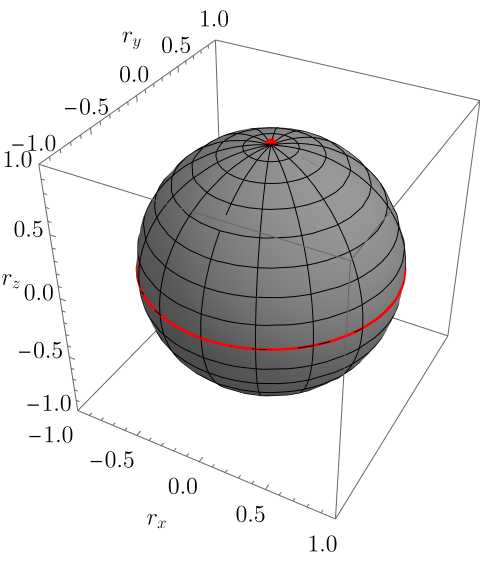
\includegraphics[width=0.9\linewidth]{chapter3/figures_special/sphere_Ising_t=0._z=0.9_p=0.5.png}
      \caption{$t=0$}
    \end{subfigure}%
    \begin{subfigure}{0.32\textwidth}
      \centering
      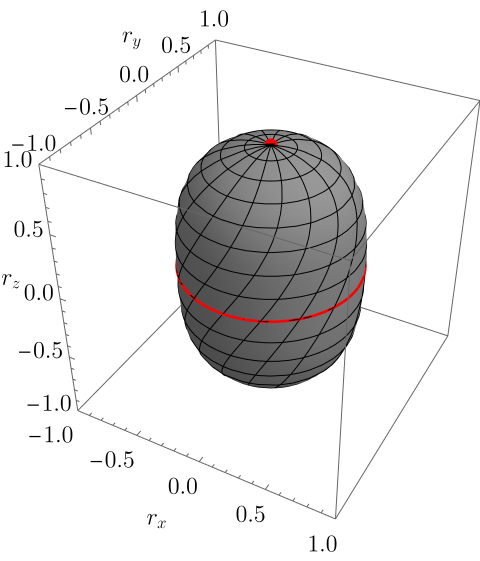
\includegraphics[width=0.9\linewidth]{chapter3/figures_special/sphere_Ising_t=0.5_z=0.9_p=0.5.png}
      \caption{$t=0.5$}
    \end{subfigure}
    \begin{subfigure}{0.32\textwidth}
      \centering
      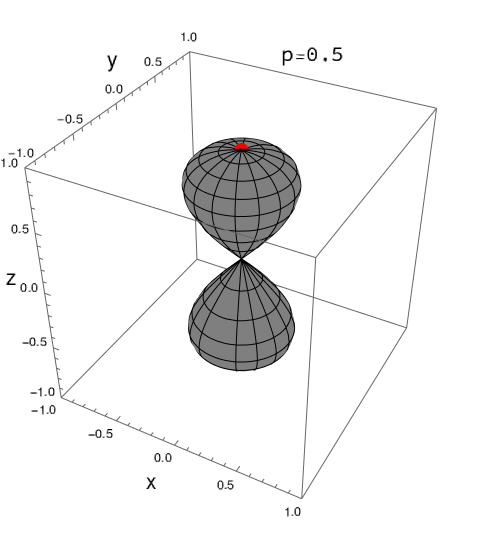
\includegraphics[width=0.9\linewidth]{chapter3/figures_special/sphere_Ising_t=1._z=0.9_p=0.5.png}
      \caption{$t=1$}
    \end{subfigure}
    \caption{Efecto sobre la esfera de Bloch de la dinámica efectiva inducida por el hamiltoniano de la cadena de Ising de dos partículas a diferentes tiempos $t$. Nótese que el desfasamiento sólo se completa para estados tales que $r_{z}=0$.\label{fig:Ising_p0.5_Sequence}}
\end{figure}



Como es natural, la expresión de la dinámica efectiva se vuelve cada vez más complicada y menos informativa conforme se aumenta el número de partículas. La dinámica unitaria general para la cadena de Ising cerrada sin campo transversal es
\begin{align}
    \mcU_{t}=&\qty(\cos^{n}(\omega t)+(-\rmi)^{n}\sin^{n}(\omega t))\Id\nonumber\\ 
    &+\sum_{k=2}^{n-1}(-\rmi)^{n-k}\cos^{k}(\omega t)\sin^{n-k}(\omega t)\sum_{k_{1}<k_{2}}(\pauli{3,k_{1}}\pauli{3,k_{1}+1})(\pauli{3,k_{2}}\pauli{3,k_{2}+1}),\nonumber
\end{align}
mientras que para la cadena de Ising abierta es
\begin{align}
    \mcU_{t}=&\cos^{n}(\omega t)\Id+(-\rmi)^{n}\sin^{n}(\omega t)\pauli{3,1}\pauli{3,n}\nonumber\\ 
    &+\sum_{k=2}^{n-1}(-\rmi)^{n-k}\cos^{k}(\omega t)\sin^{n-k}(\omega t)\sum_{k_{1}<k_{2}}(\pauli{3,k_{1}}\pauli{3,k_{1}+1})(\pauli{3,k_{2}}\pauli{3,k_{2}+1}).\nonumber
\end{align}
Si se quisiera hallar la dinámica efectiva siguiendo el mismo procedimiento que se ha utilizado hasta ahora, esta tendría términos dependientes de los valores esperados de cadenas de Pauli $\pauli{3}^{\vec{j}}$, donde $\vec{j}$ tiene $n-1$ entradas, cosa que se traduce en un aumento exponencial en el número de términos conforme crezca $n$. Aunque en este trabajo no se buscarán dichas expresiones, es posible usar calculadoras simbólicas para obtener visualizaciones de dichas dinámicas efectivas. 

\begin{figure}
    \centering
    \begin{subfigure}[b]{0.475\textwidth}
        \centering
        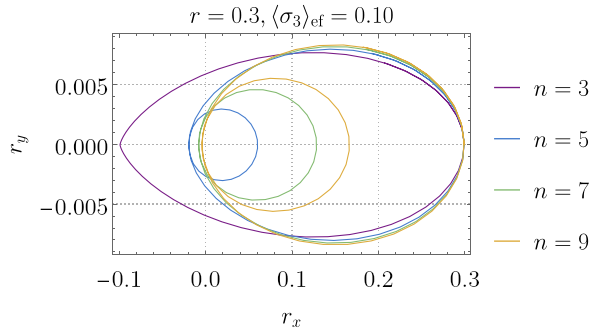
\includegraphics[width=\textwidth]{chapter3/figures_special/Ising_Boltz_r=0.3_z=0.10.png}
    \end{subfigure}
    \hfill
    \begin{subfigure}[b]{0.475\textwidth}  
        \centering 
        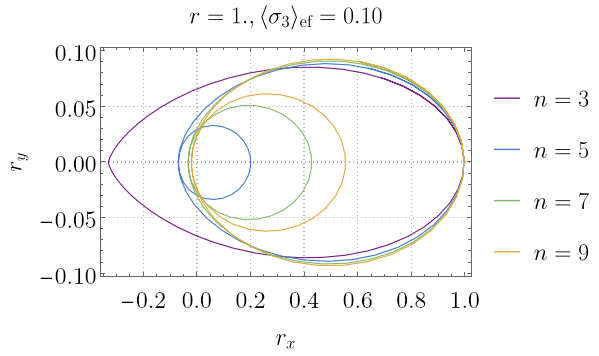
\includegraphics[width=\textwidth]{chapter3/figures_special/Ising_Boltz_r=1._z=0.10.png}
    \end{subfigure}
    \caption{Evolución del vector de Bloch de un estado efectivo inicial tal que $r_{z}=0.1$ en el régimen de Boltzmann, inducida por el hamiltoniano de la cadena de Ising abierta de $n$ partículas, para diferentes valores de $n$ y dos valores distintos del radio de Bloch inicial $r_{\ef}$.}
    \label{fig:OpenIsingBoltz}
\end{figure}

La figura \ref{fig:OpenIsingBoltz} muestra la misma evolución pero en el caso del régimen de Boltzmann. Nótese que la forma de la evolución no parece depender del radio de Bloch inicial, pero que cambia considerablemente conforme aumenta el número de partículas $n$. Además, la evolución, lejos de ser una rotación alrededor de $r_{z}$, a cualquier tiempo $t\neq 0$ conlleva cierto grado de desfasamiento. Esto es, $r_{\ef}(t)<r_{\ef}(0)$. Queda por ser estudiado el límite $n\rightarrow\infty$, para el que parece se completa el desfasamiento.

Por otro lado, figura \ref{fig:OpenIsingPref} muestra la evolución del vector de Bloch del estado efectivo, $\vec{r}_{\ef}(t)$, en el plano $r_{z}=0.1$, en el caso del régimen preferencial, para diferentes valores de $p_{1}$. Nuevamente, el valor inicial del vector de Bloch no tiene efecto en la forma general de la evolución, por lo que solo se muestra el caso en el que el estado efectivo inicial es puro. A notarse que la dinámica se aleja cada vez más de una evolución unitaria conforme disminuye $p_{1}$ y aumenta el número de partículas $n$

\begin{figure}
    \centering
    \begin{subfigure}[b]{0.475\textwidth}
        \centering
        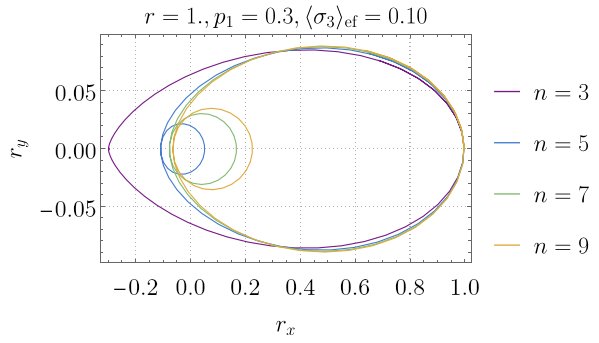
\includegraphics[width=\textwidth]{chapter3/figures_special/Ising_Pref_p1=0.3_z=0.10.png}
    \end{subfigure}
    \hfill
    \begin{subfigure}[b]{0.475\textwidth}  
        \centering 
        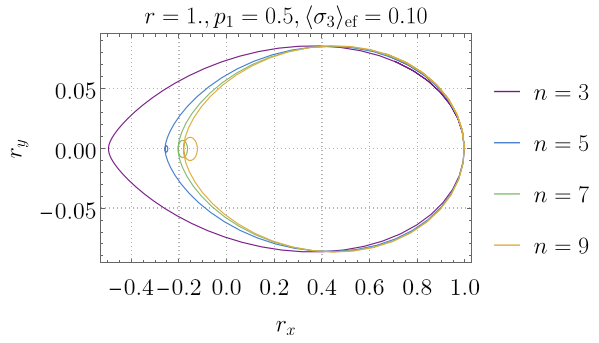
\includegraphics[width=\textwidth]{chapter3/figures_special/Ising_Pref_p1=0.5_z=0.10.png}
    \end{subfigure}
    \vskip\baselineskip
    \begin{subfigure}[b]{0.475\textwidth}   
        \centering 
        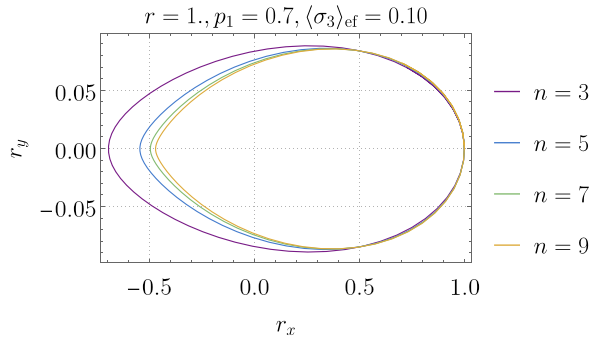
\includegraphics[width=\textwidth]{chapter3/figures_special/Ising_Pref_p1=0.7_z=0.10.png}
    \end{subfigure}
    \hfill
    \begin{subfigure}[b]{0.475\textwidth}   
        \centering 
        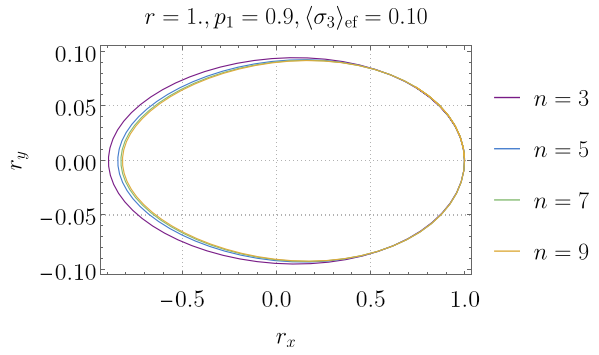
\includegraphics[width=\textwidth]{chapter3/figures_special/Ising_Pref_p1=0.9_z=0.10.png}
    \end{subfigure}
    \caption{Evolución del vector de Bloch de un estado efectivo inicial tal que $r_{z}=0.1$ en el régimen de partícula preferencial, inducida por el hamiltoniano de la cadena de Ising abierta de $n$ partículas, para diferentes valores de $n$ y cuatro valores del parámetro probabilístico asociado a la partícula preferencial, $p_{1}$.}
    \label{fig:OpenIsingPref}
\end{figure}

En ambos casos las dinámicas son no lineales, y, en algunos casos particulares parecen tener derivadas no continuas en casos particulares (ver figura \ref{fig:OpenIsingPref}, caso $n=3$).
